\subsubsection{Effective diffusivity case} \label{analytical}

Although validation against experiments could show that FESTIM is able reproduce the data with a given set of parameters, objective verification against analytical solutions is first required to ensure that the governing Equations \ref{eq:mobile} and \ref{eq:trapped} are solved correctly.

For this verification case, a 1D slab is considered with a thickness $l$.
The concentration of mobile particles was set to $c_0$ on one side of the slab and set to zero on the other side.
Only one trap is considered in this case and its density $n_1$ is homogeneously distributed.

The trapping parameter $\zeta$ is defined in \sidecite{longhurst_verification_2005} as follow:
\begin{equation}
    \zeta = \frac{\lambda^2 \: n_\mathrm{solute} \: \nu_0}{D_0 \: n_1}\exp\bigg(\frac{E_\mathrm{diff} - E_1}{k_B \: T}\bigg) + \frac{c_m}{n_1}
\end{equation}

In our case, we choose the detrapping energy $E_1$, the concentration $c_0$ and the temperature $T$ so that $\zeta \gg \frac{c_m}{n_1}$.
This is known as the \textit{effective diffusivity regime} where the diffusion is almost identical to the case where there are no traps.
The coefficient $D$ is then replaced by an effective diffusion coefficient:
\begin{equation}
    D_\mathrm{eff} = \frac{D}{1+\frac{1}{\zeta}}
\end{equation}
The particle flux at the background surface is expressed in $\SI{}{H.m^{-2}.s^{-1}}$ and finally defined in \sidecite{longhurst_verification_2005} by:
\begin{equation}
    \varphi_H(t) = \frac{c_0 D}{l}\bigg[1+2\sum_{m=1}^{\infty}(-1)^m \exp\bigg(-m^2\frac{\pi^2 \:D_\mathrm{eff} \: t}{l^2}\bigg)\bigg]
\label{eq:flux analytical}
\end{equation}
All the parameters are defined in Table \ref{tab:parameters analytical verification}.
These parameters have been chosen for the sake of verification and do not necessarily represent realistic conditions as verification is a mathematical exercise.
\begin{table}
    \centering
    \begin{tabular}{p{2.3cm} p{2cm} r}
        Parameter & Units & Value \\
        \hline
        \\
        $\rho$ & $\si{m^{-3}}$ &$\SI{3.16e22}{}$ \\
        $n_1$ & & $\SI{1.00e-1}{} \rho$ \\
        $c_0$ & & $\SI{1.00e-4}{} \rho$\\
        $n_\mathrm{solute}$ & & $2 \:\rho$\\
        \\
        $E_1$ & $\si{eV}$ & $\SI{8.6e-3}{}$ \\
        $E_\mathrm{diff}$ & & $0$ \\
        \\
        $\lambda$ & $\si{m}$ & $\SI{3.16e-8}{}$  \\
        $l$ & & $\SI{5e-5}{}$\\
        \\
        $T$ & $\si{K}$ & 1000 \\
        \\
        $t_f$ & $\si{s}$ & \SI{e-8}{} \\
        $\nu_0$ & $\si{s^{-1}}$ & $\SI{e13}{}$ \\
        $D_0$ & $\si{m^2.s^{-1}}$ & $1$ \\
        \\
    \end{tabular}
    \caption{Parameters used for the analytical verification}
    \label{tab:parameters analytical verification}
\end{table}
One can notice on Figure \ref{fig:FESTIM vs analytical} that the numerical results are in good agreement with the analytical solution.
The maximum error between analytical and numerical solutions is calculated to be \SI{6.56e20}{H.m^{-2}.s^{-1}} with 50000 piecewise linear elements (P1) which corresponds to \SI{1}{\%} of the maximum value.
According to finite elements theory, this value will decrease with the stepsize and with the element size.
\begin{figure}
    \centering
    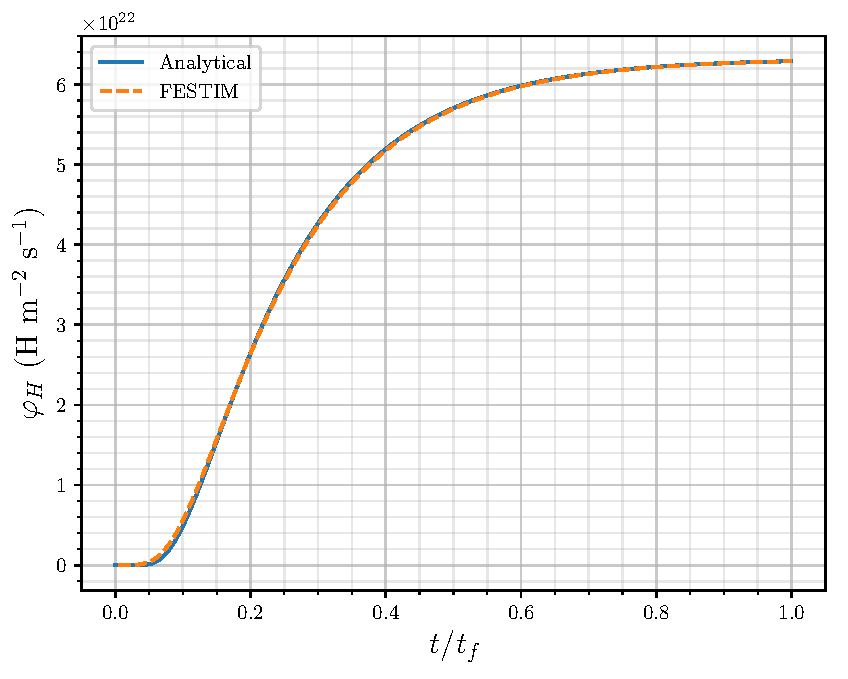
\includegraphics[width=\linewidth]{Figures/Chapter3/FESTIM_vs_analytical.pdf}
    \caption{Temporal evolution of the particle flux $\varphi_H$ ($t_f = \SI{e-8}{s}$)}
    \label{fig:FESTIM vs analytical}
\end{figure}
\subsubsection{Analytical verification using MMS} \label{mms}

To unravel the complexity of governing equations, the Method of Manufactured Solutions (MMS) is often used \sidecite{dudson_verification_2016, roache_code_2002}.
Manufactured solutions are exact solutions that have been modified with additional source terms.
The sets of source terms and boundary conditions obtained are then fed into FESTIM and the error is measured.


At this extent the following manufactured solutions are chosen:
\begin{equation}
    \begin{cases}
    c_{m_D} = 1 + x^2 + \sin(t) \\
    c_{{t,1}_D} = 1 + x^2 + \cos(t)
    \end{cases}
    \label{eq: manufactured solutions}
\end{equation}

By combining Equations \ref{eq:mobile}, \ref{eq:trapped} and \ref{eq: manufactured solutions}, one can obtain the following source terms:
\begin{equation}
    \begin{cases}
    f = \cos(t) - \sin(t) - 2D \\
    g_1 = \nu_1 c_{{t,1}_D} - \nu_m c_{m_D} ( n_1 - c_{{t,1}_D}) - \sin(t)
    \end{cases}
    \label{eq:sources}
\end{equation}

where $g_1$ is an additional source term in Equation \ref{eq:trapped}.
The Dirichlet boundary conditions for $c_m$ and $c_{t,1}$ are:

\begin{equation}
    \begin{cases}
    c_m = 1 + x^2 + \sin(t) \quad \text{on } \partial \Omega \\
    c_{t,1} = 1 + x^2 + \cos(t) \quad \text{on } \partial \Omega 
    \end{cases}
\end{equation}
where $\partial\Omega$ is the boundary of the domain.
Finally, initial values for $c_m$ and $c_{t,i}$ are:
\begin{equation}
    \begin{cases}
    c_m(t=0) = 1 + x^2 \\
    c_{t,1}(t=0) = 2 + x^2
    \end{cases}
\end{equation}
Once all these parameters are fed into FESTIM, one can easily compare the computed solution with the exact solution in Equation \ref{eq: manufactured solutions}.
The L2-norm $E_{c_m}$ can then be calculated as follow:
\begin{equation}
    E_{c_m} = \sqrt{\int_\Omega(c_{m_D} - c_m)^2dx}
\end{equation}
The evolution of $E_{c_m}$ as function of the element size $h$ is shown on Figure \ref{fig:error vs h}.
One can notice that $E_{c_m}$ increases as $A\cdot h^k$.
This is known as the \textit{asymptotic regime} and the coefficient $k$ is called the convergence rate.
$k$ typically tends to N+1 as $h$ approaches $0$, $N$ being the order of the finite elements.
In this simulation, $k$ approaches $2$ as expected since elements of order $1$ have been used.

\begin{figure}
    \centering
    \includegraphics[width=1\linewidth]{"Figures/Chapter3/L2 error on Cm vs h"}
    \caption{Evolution of the L2 norm of the error as function of element size h}
    \label{fig:error vs h}
\end{figure}

The results of the verification cases studied in Sections \ref{analytical} and \ref{mms} show that FESTIM reliably solves the governing Equations \ref{eq:mobile} and \ref{eq:trapped}.
It has also been shown that the convergence rate is in accordance with the theory of finite elements meaning that the code is free of errors that could lead to unreliable results in the future.
Validation can then be performed to ensure that the MRE model described in Section \ref{description_H_transport_model} can be used to reproduce experimental results.

\subsection{Conservation of chemical potential verification}
To ensure the implementation of the interface model in FESTIM is error free, analytical verification is required since physical trend tests are not rigorous enough. The verification process aims at checking the code is correctly solving the governing Equations \ref{eq: flux conservation}, \ref{eq: c/s conservation}, \ref{eq: diffusion equation} and \ref{eq: diffusion equation changed}.
To this end, two methods were used: the Method of Exact Solutions (MES) and the Method of Manufactured Solutions (MMS).
It is worth noting that these two methods do not require to be physically realistic since this is a purely mathematical exercise.
In practice, not having real life properties or realistic domain sizes can even facilitate the construction of a general test case and therefore ease the results reproduction by others.
A complete H transport problem would include coupling with trapping/detrapping (as in Section \ref{iter case}).
The implementation of the trapping/detrapping coupling in FESTIM has already been analytically verified in \sidecite{delaporte-mathurin_finite_2019} therefore this Section will only focus on verifying the solving of Equations \ref{eq: flux conservation}, \ref{eq: c/s conservation}, \ref{eq: diffusion equation} and \ref{eq: diffusion equation changed}.

\subsubsection{Method of Exact Solutions (MES)}

\begin{figure*} [h]
    \centering
    \begin{subfigure}{0.5\linewidth}
        \centering
        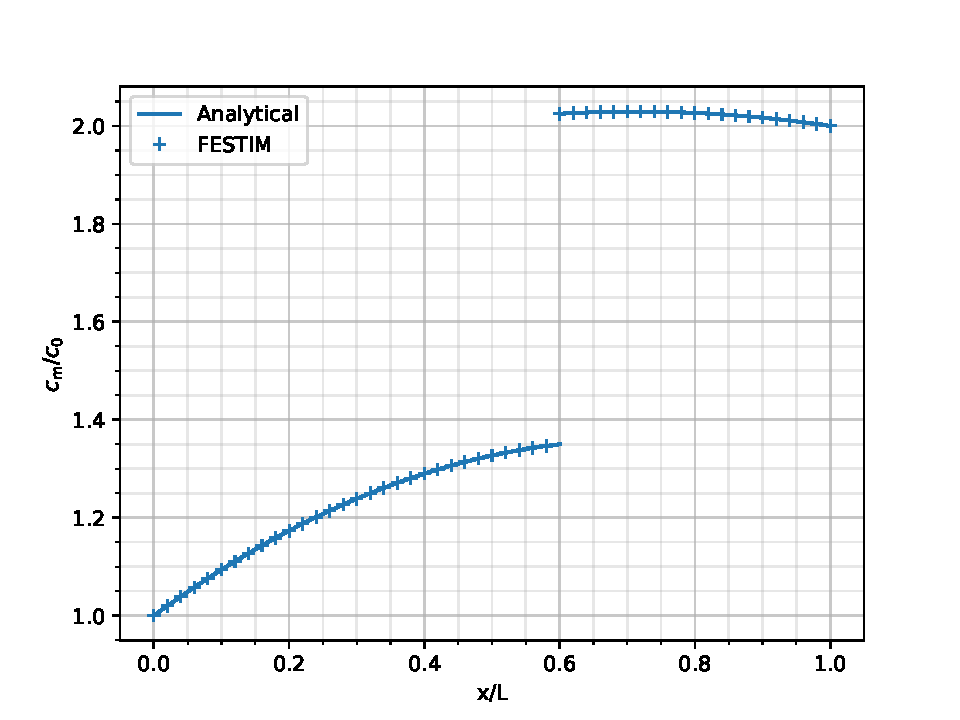
\includegraphics[width=\linewidth]{Figures/Chapter3/monoblocks/interface_condition/out_MES_case1.pdf}
        \caption{Case 1: $\alpha = 2$, $\beta = 1.5$, $\gamma=0.6$, $\tilde{c}_L = 2$, $\tilde{f}=1$}
    \end{subfigure}%
    % \hfill
    \begin{subfigure}{0.5\linewidth}
        \centering
        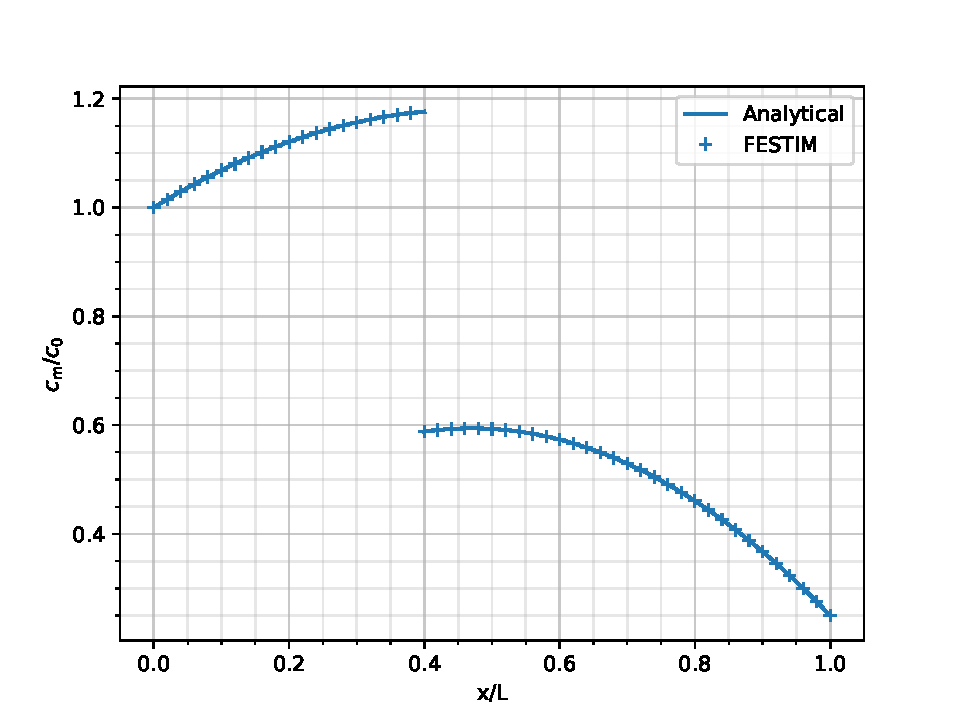
\includegraphics[width=\linewidth]{Figures/Chapter3/monoblocks/interface_condition/out_MES_case2.pdf}
        \caption{Case 2:  $\alpha = 1.5$, $\beta = 0.5$, $\gamma=0.4$, $\tilde{c}_L = 0.25$, $\tilde{f}=2$}
    \end{subfigure}
    \caption{Concentration profiles simulated by FESTIM against analytical solutions.}
    \label{fig:comparison MES}
\end{figure}*

The uni-dimensional test case considered in this Section was made of two subdomains $\Omega_1$ and $\Omega_2$ and is described as follow:
\begin{subequations}
\begin{align}
    \Omega &= [0, L] = \Omega_1 \cup \Omega_2 \\
    \Omega_1 &= [0, x_\mathrm{int}] \\
    \Omega_2 &= [x_\mathrm{int}, L] \\
    D &= \begin{cases}
        D_1,& \text{ in } \Omega_1\\
        D_2,& \text{ in } \Omega_2
    \end{cases} \\
    S &= \begin{cases}
        S_1,& \text{ in } \Omega_1\\
        S_2,& \text{ in } \Omega_2
    \end{cases}
\end{align}
\end{subequations}

The following dimensionless quantities are introduced:
\begin{subequations}
    \begin{align}
        \tilde{c}_\mathrm{m} &= c_\mathrm{m} / c_0\\
        \tilde{x} &= x / L \\
        \tilde{f} &= f \frac{L^2}{D_\mathrm{eq} c_0} \\
        \alpha &= D_2/D_1 \\
        \beta &= S_2/S_1 \\
        \gamma &= x_\mathrm{int}/L\\
    \end{align} 
\end{subequations}
where $D_\mathrm{eq} = (D_1 D_2)^{1/2}$.

By integrating Equation \ref{eq: diffusion equation} and assuming steady-state (\textit{i.e.} $\partial c/\partial t=0$), one can obtain the following dimensionless form:

\begin{equation}
        \tilde{c}_\mathrm{m}= 
\begin{cases}
    -\frac{1}{2}\alpha^{1/2}\tilde{f} \tilde{x}^2 + a_1 \tilde{x} + b_1,& \text{ in } \Omega_1\\
    -\frac{1}{2}\alpha^{-1/2}\tilde{f} \tilde{x}^2 + a_2 \tilde{x} + b_2,& \text{ in } \Omega_2
\end{cases}
\label{eq:MES c}
\end{equation}

% \begin{equation}
%         c_\mathrm{m}= 
% \begin{cases}
%     \frac{-f}{2D_1} x^2 + a_1 x + b_1,& \text{ in } \Omega_1\\
%     \frac{-f}{2D_2} x^2 + a_2 x + b_2,& \text{ in } \Omega_2
% \end{cases}
% \tilde
% \label{eq:MES c}
% \end{equation}
where $a_1$, $b_1$, $a_2$, $b_2$ are the unknowns of the problem to be determined.
The boundary conditions and the equilibrium law at the interface are defined as:
\begin{subequations} \label{eq: bcs MES}
\begin{align} 
        \tilde{c}_\mathrm{m}(\tilde{x}=0) & = 1 \\
        \tilde{c}_\mathrm{m}(\tilde{x}=1) & =  \tilde{c}_L \\
        \tilde{c}_\mathrm{m}^-(\tilde{x}=\gamma) & =  \beta \; \tilde{c}_\mathrm{m}^+(\tilde{x}=\gamma)\\
        \nabla \tilde{c}_\mathrm{m}^-(\tilde{x}=\gamma) & =  \alpha \nabla \tilde{c}_\mathrm{m}^+(\tilde{x}=\gamma)
\end{align}
\end{subequations}


Equation \ref{eq:MES c} can be solved with these constraints and coefficients describing $c_\mathrm{m}$ therefore read:

% \begin{align}
%     \begin{split}
%         a_1 &= \frac{- 2 D_{1} D_{2} S_{2} c_{0} + D_{1} S_{1} \left(2 D_{2} c_L - f L^{2}\right) + f x_\mathrm{int}^{2} \left(D_{1} S_{1} - D_{2} S_{2}\right)}{2 D_{1} \left(D_{1} S_{1} L - D_{1} S_{1} x_\mathrm{int} + D_{2} S_{2} x_\mathrm{int}\right)}  \\
%         b_1 &= c_0 \\
%         a_2 &= \frac{- 2 D_{1} D_{2} S_{2} c_{0} + D_{1} S_{1} \left(2 D_{2} c_{L} - f L ^{2}\right) + f x_\mathrm{int}^{2} \left(D_{1} S_{1} - D_{2} S_{2}\right)}{2 D_{2} \left(D_{1} S_{1} L  - D_{1} S_{1} x_\mathrm{int} + D_{2} S_{2} x_\mathrm{int}\right)}\\
%         b_2 &= \frac{2 D_{1} D_{2} L S_{2} c_{0} - x_\mathrm{int} \left(D_{1} S_{1} - D_{2} S_{2}\right) \left((L f x_\mathrm{int} +  \left(2 D_{2} c_{L} - L^{2} f\right)\right)}{2 D_{2} \left(D_{1} S_{1} L - D_{1} S_{1} x_\mathrm{int} + D_{2} S_{2} x_\mathrm{int}\right)} 
%     \end{split}
% \end{align}


\begin{align}
    \begin{split}
        a_1 &= a_0 \; \alpha^{1/2}  \\
        b_1 &= 1 \\
        a_2 &= a_0 \; \alpha^{-1/2}\\
        b_2 &= \tilde{c}_L + \frac{1}{2} \alpha^{-1/2} \tilde{f} - a_2 \\
        a_0 &= \frac{2 \alpha^{1/2}( \tilde{c}_L - \beta) + \tilde{f} \gamma^{2} ( 1 - \alpha \beta)}{2 \left( 1  - \gamma + \alpha \beta \gamma \right)} \\
    \end{split}
    \label{eq: MES c coefficients}
\end{align}

It is worth noting that when $\beta=1$ (\textit{i.e.} $S_1 = S_2 = S$) the solution becomes independent of $S$ and {$c_\mathrm{m}^{-}(x_\mathrm{int}) = c_\mathrm{m}^{+}(x_\mathrm{int})$}.
Moreover, when $\alpha = 1$ (\textit{i.e.} $D_1 = D_2 = D$), then $a_1 = a_2 = a_0$ which is the solution for steady-state diffusion in a mono-material.

The solution computed by FESTIM was found to be in very good agreement with the analytical solution for several test cases (see Figure \ref{fig:comparison MES}).

 
However, this method does not exercise all the terms in the governing Equation \ref{eq: diffusion equation changed}.
For instance, this analytical solution is only uni-dimensional, steady state is assumed and material properties are constant within the materials.
Having an exact solution from an analytical resolution for a general problem (multidimensional, transient, heterogeneous material properties, etc...) is often complex.
In order to exercise all these terms, the Method of Manufactured Solutions (MMS) will therefore be employed for it offers a good alternative to unravel these complexities.

\subsubsection{Method of Manufactured Solutions (MMS)}

The goal of Method of Manufactured Solutions (MMS) is to have an exact solution which is general enough to exercise all the terms of the governing equations.
This method also allows to test the implementation of the FESTIM code on a multidimensional problem.

The domain $\Omega$ for this test problem is a unit square composed of two subdomains $\Omega_1$ and $\Omega_2$ (see Equation \ref{eq: MMS domain}).
\begin{subequations} \label{eq: MMS domain}
\begin{align}
    \Omega &= [0, 1] \times [0, 1] \\
    \Omega_1 &= [0, x_\mathrm{int}] \times [0, 1] \\
    \Omega_2 &= [x_\mathrm{int}, 1] \times [0, 1] \\
\end{align}
\end{subequations}
In order to unravel the complexity of an analytical resolution of the direct problem, a manufactured solution $c_M$ was constructed (see Equation \ref{eq: manufactured solution}) and the problem was solved backwards.

\begin{equation}
        c_M= 
\begin{cases}
    c_{M1},& \text{ on } \Omega_1\\
    \frac{S_2}{S_1} \cdot c_{M1},& \text{ on } \Omega_2
\end{cases}
\label{eq: manufactured solution}
\end{equation}
where $c_{M1} = 2 + \cos(2\pi x) \cdot \cos(2\pi y) + t$

It is worth noting that, when choosing a manufactured solution, one must ensure it satisfies all the governing equations (especially Equations \ref{eq: flux conservation} and \ref{eq: c/s conservation}).
In our case, $c_M$ ensures the flux conservation at the interface and the continuity of the quantity $c_\mathrm{m}/S$.

Properties are assumed time and space dependent in order to test every portion of the code (see Equation \ref{eq: MMS properties}).
\begin{subequations}
    \begin{align}
        D_1(x, y, t) & =  D_{1_0} \exp(-E_{D_1}/(k_B \cdot T(x,y, t) )) \\
        D_2(x, y, t) & =  D_{2_0} \exp(-E_{D_2}/(k_B \cdot T(x,y, t) )) \\
        S_1(x, y, t) & =  S_{1_0} \exp(-E_{S_1}/(k_B \cdot T(x,y, t) )) \\
        S_2(x, y, t) & =  S_{2_0} \exp(-E_{S_2}/(k_B \cdot T(x,y, t) )) \\
        T(x, y, t) & = 500 + 30 \cos(2\pi x) \cos(2 \pi y) \cos(2 \pi t)
\end{align} \label{eq: MMS properties}
\end{subequations}
with ${k_B = \SI{8.617e-5}{eV.K^{-1}}}$ the Boltzmann constant, $D_{1_0} = 1$, $E_{D_1} = 0.1$, $D_{2_0} = 2$, $E_{D_2} = 0.2$, $S_{1_0} = 1$, $E_{S_1} = 0.1$, $S_{2_0} = 2$ and $E_{S_2} = 0.2$.
The temperature $T$ varies around \SI{500}{K} so that, given the activation energies, properties do not approach zero.

By injecting the manufactured solution $c_M$ into the governing Equation \ref{eq: diffusion equation}, the source term can be expressed as:
\begin{align}
    f(x, y, t) &= \frac{\partial c_M}{\partial t} - \vec{\nabla} \cdot\left(D(x, y)
    \vec{\nabla}c_M\right) \nonumber \\
    &= \begin{cases}
        \frac{\partial c_{M_1}}{\partial t} - \vec{\nabla} \cdot\left(D_1(x, y)
    \vec{\nabla}c_{M_1}\right),& \text{ on } \Omega_1\\
    \frac{\partial c_{M_2}}{\partial t} - \vec{\nabla} \cdot\left(D_2(x, y)
    \vec{\nabla}c_{M_2}\right),& \text{ on } \Omega_2\\
    \end{cases}
\end{align}

The source term $f$ was then fed into FESTIM alongside with the initial and boundary conditions described below:
\begin{subequations}
    \begin{align}
        c_\mathrm{m}(x, y, t) &= c_M(x, y, t), \text{ on } \partial \Omega \\
        c_\mathrm{m}(x, y, t=0) &= c_M(x, y, t=0), \text{ on } \Omega
    \end{align}
\end{subequations}

The computed solution $c_\mathrm{comp}$ can then be compared with the manufactured solution $c_M$ in order to quantitatively measure the numerical error.
After running the MMS process, the computed solution and the manufactured solution were in very good agreement at several arbitrarily chosen times of simulation (see Figure \ref{fig: results MMS}).
% The stepsize was $\Delta t=0.01$.
The absolute difference between the manufactured solution and the computed one was found to be zero on the boundary and maximum at the interface between the two materials.
This is explained by the Dirichlet boundary conditions enforcing the computed solution on the boundary.
This difference decreases by increasing the mesh refinement and decreasing the stepsize.
Nonetheless, the error was found to remain orders of magnitude lower than the actual solution.

\begin{figure*}
    \centering
    \begin{subfigure}{0.33\linewidth}
        \centering
        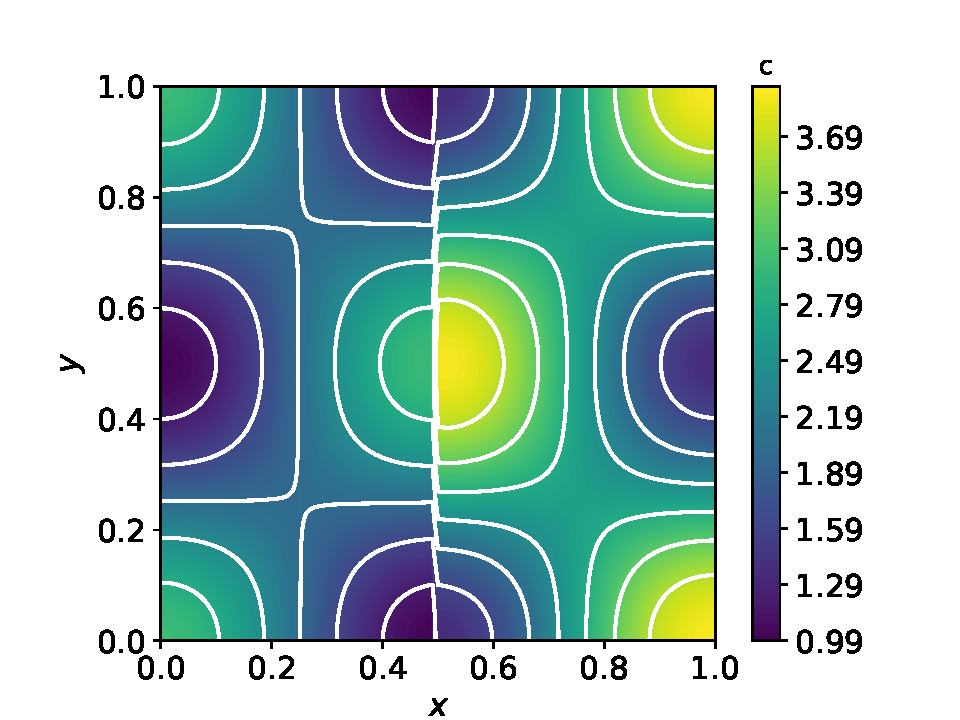
\includegraphics[width=\linewidth]{Figures/Chapter3/monoblocks/interface_condition/u_computed_t0.01.pdf}
        \caption{Computed solution $c_\mathrm{comp}(t=0.01)$}
    \end{subfigure}%
    \begin{subfigure}{0.33\linewidth}
        \centering
        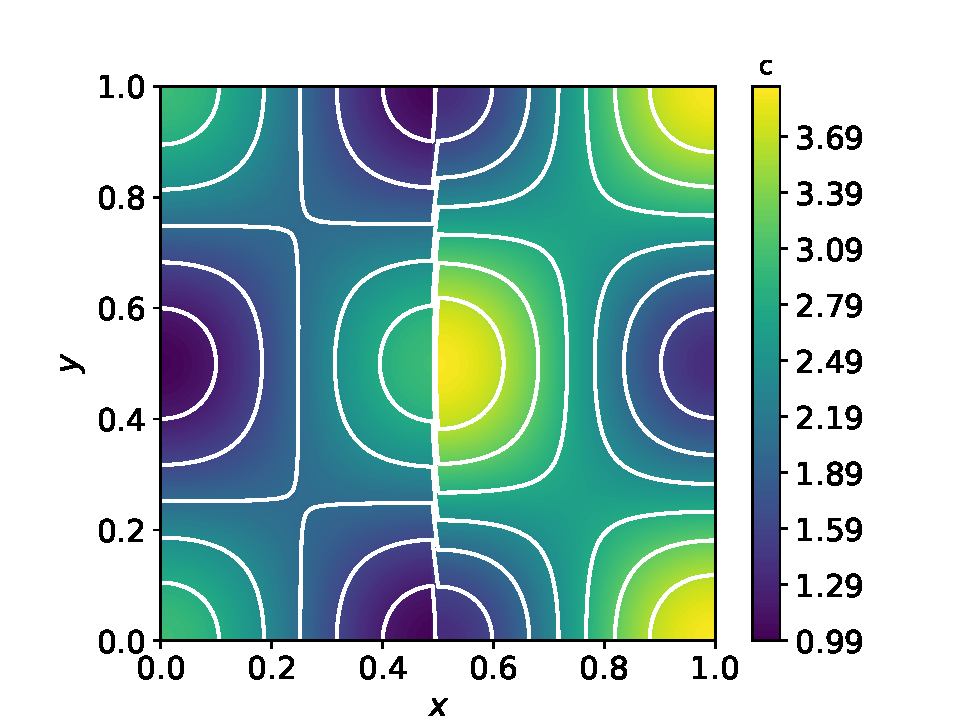
\includegraphics[width=\linewidth]{Figures/Chapter3/monoblocks/interface_condition/u_exact_t0.01.pdf}
        \caption{Exact solution $c_M(t=0.01)$}
    \end{subfigure}%
    \begin{subfigure}{0.33\linewidth}
        \centering
        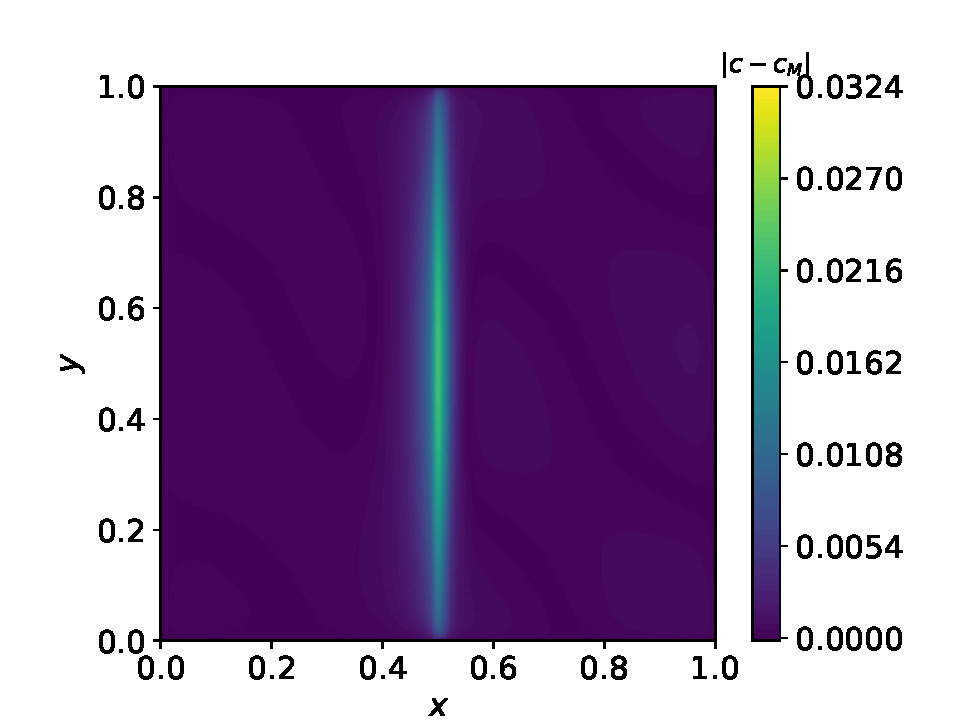
\includegraphics[width=\linewidth]{Figures/Chapter3/monoblocks/interface_condition/diff_t0.01.pdf}
        \caption{Absolute difference}
    \end{subfigure}
    \begin{subfigure}{0.33\linewidth}
        \centering
        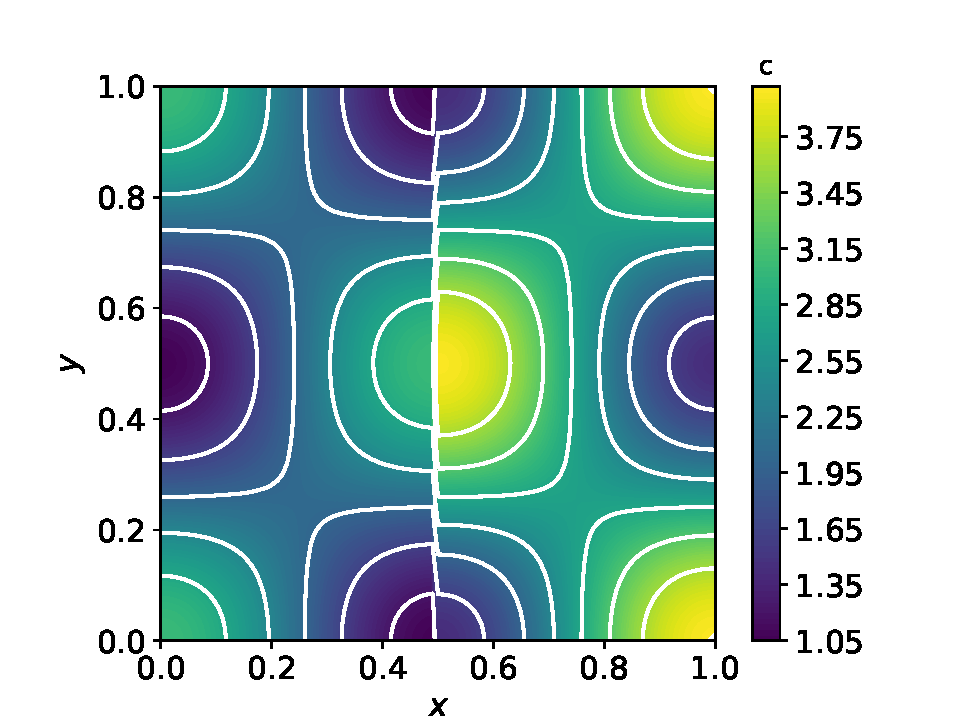
\includegraphics[width=\linewidth]{Figures/Chapter3/monoblocks/interface_condition/u_computed_t0.06.pdf}
        \caption{Computed solution $c_\mathrm{comp}(t=0.06)$}
    \end{subfigure}%
    \begin{subfigure}{0.33\linewidth}
        \centering
        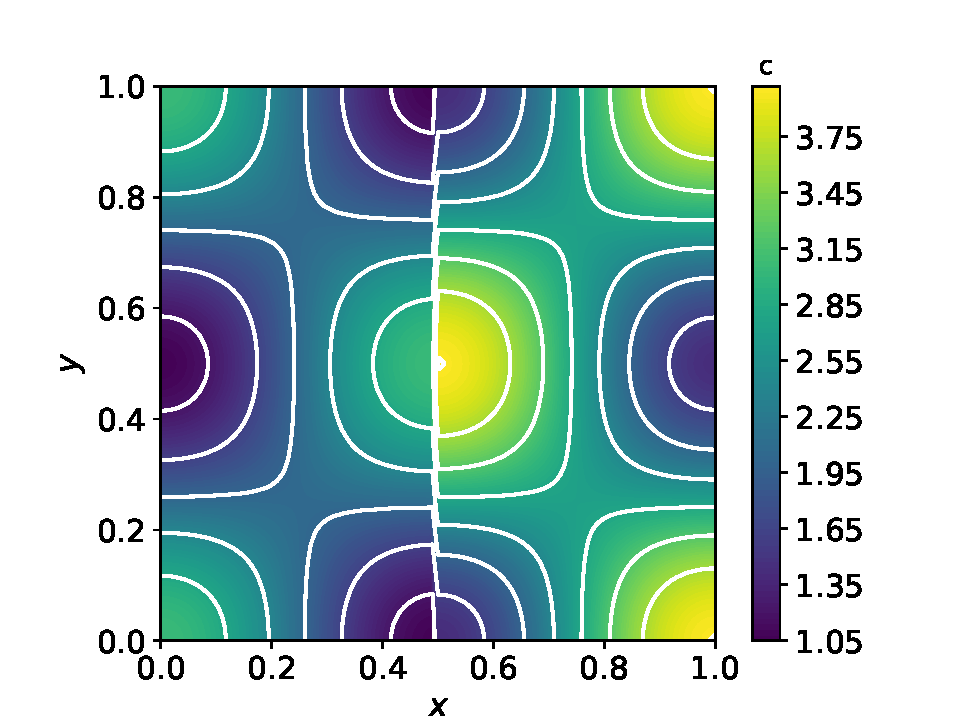
\includegraphics[width=\linewidth]{Figures/Chapter3/monoblocks/interface_condition/u_exact_t0.06.pdf}
        \caption{Exact solution $c_M(t=0.06)$}
    \end{subfigure}%
    \begin{subfigure}{0.33\linewidth}
        \centering
        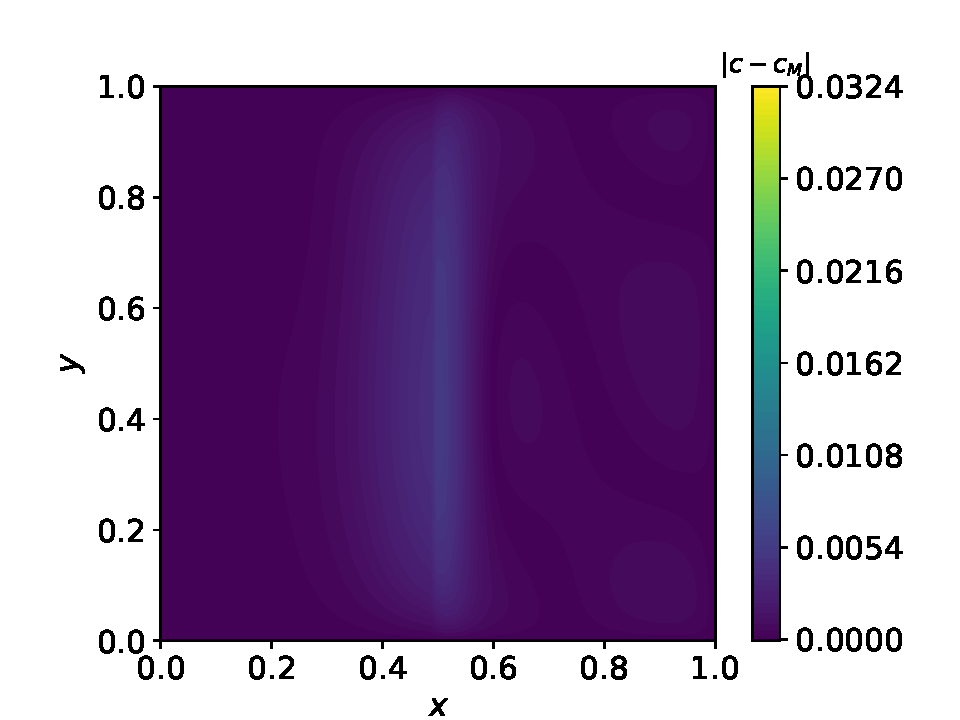
\includegraphics[width=\linewidth]{Figures/Chapter3/monoblocks/interface_condition/diff_t0.06.pdf}
        \caption{Absolute difference}
    \end{subfigure}
    \caption{Comparison of concentration fields simulated by FESTIM with manufactured solutions}
    \label{fig: results MMS}
\end{figure*}


% The chemical potential continuity at interface is not directly equivalent to a concentration continuity (see Equation \ref{eq: cconservation})  since the chemical potential in a reference state is not the same in different materials \sidecite{kirchheim_25_2014}, as the lattice site concentration.
% \begin{equation}
%             c^- = c^+  \label{eq: cconservation} 
% \end{equation}

\subsubsection{Heat transfer}

TODO: verification of the heat transfer equation
2D case